\documentclass[11pt,a4paper]{article}

\usepackage[margin=1in]{geometry}
\usepackage[T1]{fontenc}
\usepackage[utf8]{inputenc}
\usepackage{lmodern}
\usepackage{setspace}
\usepackage{booktabs}
\usepackage{longtable}
\usepackage{array}
\usepackage{graphicx}
\usepackage{float}
\usepackage{hyperref}
\usepackage{xcolor}
\usepackage{tikz}
\usetikzlibrary{arrows.meta,positioning,shapes.geometric,calc}

\hypersetup{
  colorlinks=true,
  linkcolor=black,
  urlcolor=blue,
  citecolor=blue
}

\setlength{\parskip}{0.35em}
\setlength{\parindent}{1.5em}
\onehalfspacing

\title{Music Genre Classification on FMA-Large\\
\large 61.502 Deep Learning for Enterprise (Y2026)}
\author{
Ang Kar Kin \and
Nicolas Lasch \and
Nisal Jinadasa
}
\date{\today}

\begin{document}
\begin{titlepage}
\thispagestyle{empty}
\begin{tikzpicture}[remember picture, overlay]
\draw[line width=1.2pt]
  ([xshift=1cm,yshift=-1cm]current page.north west) rectangle
  ([xshift=-1cm,yshift=1cm]current page.south east);
\end{tikzpicture}
\vspace*{\fill}
\begin{center}
\vspace*{1em}
{\LARGE \textbf{Music Genre Classification on FMA-Large}\par}
\vspace{0.4em}
{\Large 61.502 Deep Learning for Enterprise (Y2026)\par}
\vspace{1.6em}
{\Large Ang Kar Kin\par}
{\Large Nicolas Lasch\par}
{\Large Nisal Jinadasa\par}
\vspace{1.2em}
{\Large \today\par}
\vspace{2em}
{\Large \textbf{Project Repository:} \url{https://github.com/<org-or-user>/<repo>} \par}
\vspace{0.5em}
{\Large \textbf{Dataset Source:} \url{https://github.com/mdeff/fma} \par}
\end{center}
\vspace*{\fill}
\end{titlepage}
\clearpage

\tableofcontents
\clearpage

\section{Executive Summary}
This project develops and evaluates deep learning models for automatic music genre classification using the FMA-Large dataset and its official metadata. We frame the task as single-label top-genre classification and compare multiple CNN variants under a shared, reproducible protocol so that observed differences are attributable to architecture and training choices rather than split leakage or inconsistent preprocessing. The best-performing model is a residual CNN configuration (``cnn\_residual\_fullprotocol''), achieving test Macro-F1 of \textbf{0.5909} and test accuracy of \textbf{0.6780}. This model outperforms both a simpler CNN baseline and a standard CNN variant.

From an enterprise delivery perspective, this work emphasizes repeatability and traceability: fixed seeds, explicit split policies, persisted intermediate artifacts, and script-level commands for full re-runs. The final recommendation is to adopt the residual CNN as the production candidate, with monitoring for distribution shift and class-specific degradation in deployment. We also recommend retaining macro-averaged metrics in governance reporting, because they expose minority-class risks that can be hidden by overall accuracy.

\section{Background and Introduction}
Music genre tagging is a practical retrieval and recommendation problem for streaming services, music libraries, and user-facing discovery systems. Manual labeling is expensive and inconsistent, especially for large catalogs. A robust genre classifier can improve playlist quality, search relevance, and downstream personalization. The key challenge is learning discriminative audio representations under class imbalance and label noise.

In this work, we target an enterprise-style delivery: reproducible training, clear evaluation against baselines, and lightweight model consumption through an inference script. The project scope is intentionally structured around model governance needs: artifact versioning, transparent comparison between alternatives, and straightforward handoff from experimentation to inference. This allows the final model recommendation to be justified not only by one metric snapshot, but also by stability across epochs, consistency across validation and test, and diagnosability through confusion-matrix analysis.

\section{Related Work}
Audio classification pipelines commonly use time-frequency representations such as Mel spectrograms and train CNN-based classifiers. Mel features are motivated by perceptual frequency scaling and have become a standard front-end for music tagging and classification tasks \cite{choi2017transfer, defferrard2017fma}. CNN families remain competitive for spectrogram-based learning because local filters can capture timbral and rhythmic structures at multiple scales, while pooling provides partial invariance to small shifts.

Residual architectures are often preferred when task difficulty and dataset size increase because skip connections improve gradient flow and optimization stability in deeper stacks \cite{he2016resnet}. In this project, we benchmark two CNN families: a residual CNN architecture (\texttt{residual\_cnn}) and a lighter standard CNN architecture (\texttt{standard\_cnn}). We also include a baseline-style training recipe to isolate how much performance gain comes from architecture alone versus regularization and augmentation policy.

\section{Problem Formulation and Solution Overview}
The task is single-label classification of the top genre from an audio track. The input is an MP3 track from FMA-Large, and the output is one genre label among the filtered training classes. The optimization objective is to maximize Macro-F1 while maintaining competitive accuracy.

Our solution follows a consistent end-to-end pipeline. We load labeled records from FMA metadata, construct stratified train, validation, and test splits, and precompute full-track Mel spectrogram caches for efficient training. We then train CNN models using random Mel crops with class-imbalance handling, evaluate each run with multi-crop aggregation on validation and test splits, and select the final model using validation Macro-F1 before reporting test metrics.

The formulation intentionally favors robust model selection over optimistic single-pass estimates. Multi-crop evaluation is used to reduce variance from any one temporal slice, and macro-averaged metrics are prioritized to reflect class imbalance. This design supports practical deployment decisions where minority-genre quality is important for user trust and catalog coverage.

\section{Data Description}
\subsection{Dataset}
We use \texttt{fma\_large} audio files and \texttt{fma\_metadata/tracks.csv}. We retain records whose subset is \texttt{large}, with non-null top-genre labels and existing valid audio files.

\subsection{Splitting and Filtering}
We use a stratified split policy with train, validation, and test ratios of 0.8, 0.1, and 0.1. We enforce minimum class-count constraints before split construction and minimum train-count constraints for class retention. Low-support classes are dropped after policy checks when required by configuration.

\subsection{Data Caveats}
The dataset has several known caveats that affect learning difficulty. Class support is imbalanced across genres, some MP3 files contain corruption artifacts, and top-genre labels can be ambiguous for tracks with cross-genre characteristics. These caveats are consistent with the FMA creators' documentation, which highlights real-world noise and metadata complexity \cite{defferrard2017fma}. In practice, this means model evaluation must be interpreted probabilistically: performance gains are meaningful, but error-free boundaries are not expected for overlapping genres.

\section{Methodology and Implementation Details}
\subsection{Feature Pipeline}
The audio pipeline uses a sampling rate of 22050 Hz and a full-cache duration of 29 seconds per track. We extract 128 Mel bins with FFT size 2048 and hop length 512. Both training and evaluation use 5-second crops, while evaluation aggregates predictions across multiple crops for stability.

Feature standardization is applied per crop to stabilize optimization and reduce sensitivity to global loudness differences. Precomputing Mel features also reduces repeated I/O and FFT overhead during training, making multi-run experiments feasible under limited compute budgets. This design choice is important for fair variant comparison, since each architecture is trained under comparable data throughput conditions.

\subsection{Model Variants}
We train three model variants under a shared protocol. The \texttt{cnn\_standard\_base\_fullprotocol} run uses \texttt{standard\_cnn} without augmentation. The \texttt{cnn\_residual\_fullprotocol} run uses \texttt{residual\_cnn} with augmentation enabled. The \texttt{cnn\_standard\_aug\_fullprotocol} run uses \texttt{standard\_cnn} with augmentation enabled, which isolates the impact of the training recipe from architecture choice.

\subsection{Architecture Diagrams}
The \texttt{standard\_cnn} stacks convolution, normalization, nonlinearity, pooling, and dropout blocks sequentially. The \texttt{residual\_cnn} uses residual blocks with identity shortcuts so each block learns a residual mapping and adds it to a skip path before activation.

\begin{figure}[H]
\centering
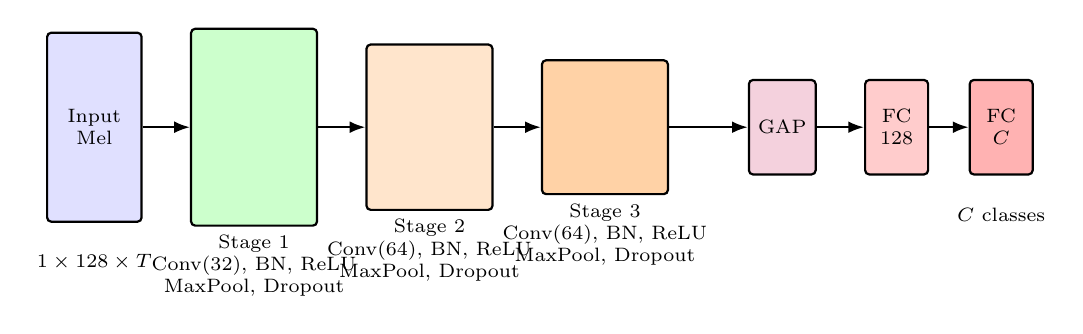
\begin{tikzpicture}[
  node distance=7mm and 6mm,
  every node/.style={font=\scriptsize},
  stage/.style={draw=black, rounded corners=1.5pt, thick, minimum width=16mm, minimum height=22mm, align=center, fill=orange!20},
  io/.style={draw=black, rounded corners=1.5pt, thick, minimum width=12mm, minimum height=24mm, align=center, fill=blue!12},
  head/.style={draw=black, rounded corners=1.5pt, thick, minimum width=8mm, minimum height=10mm, align=center, fill=purple!18},
  arr/.style={-{Latex[length=2mm]}, thick}
]
\node[io] (in) {Input\\Mel};
\node[stage, right=of in, minimum height=25mm, fill=green!20] (s1) {};
\node[stage, right=of s1, minimum height=21mm, fill=orange!20] (s2) {};
\node[stage, right=of s2, minimum height=17mm, fill=orange!35] (s3) {};
\node[head, right=10mm of s3, minimum height=12mm] (gap) {GAP};
\node[head, right=6mm of gap, minimum height=12mm, fill=red!20] (fc1) {FC\\128};
\node[head, right=5mm of fc1, minimum height=12mm, fill=red!30] (fc2) {FC\\$C$};

\draw[arr] (in) -- (s1);
\draw[arr] (s1) -- (s2);
\draw[arr] (s2) -- (s3);
\draw[arr] (s3) -- (gap);
\draw[arr] (gap) -- (fc1);
\draw[arr] (fc1) -- (fc2);

\node[align=center] at ($(in.south)+(0,-5mm)$) {$1 \times 128 \times T$};
\node[align=center] at ($(s1.south)+(0,-5mm)$) {Stage 1\\Conv(32), BN, ReLU\\MaxPool, Dropout};
\node[align=center] at ($(s2.south)+(0,-5mm)$) {Stage 2\\Conv(64), BN, ReLU\\MaxPool, Dropout};
\node[align=center] at ($(s3.south)+(0,-5mm)$) {Stage 3\\Conv(64), BN, ReLU\\MaxPool, Dropout};
\node[align=center] at ($(fc2.south)+(0,-5mm)$) {$C$ classes};
\end{tikzpicture}
\caption{Standard CNN architecture (\texttt{standard\_cnn}) used in baseline and augmentation runs.}
\label{fig:arch-standard}
\end{figure}

\begin{figure}[H]
\centering
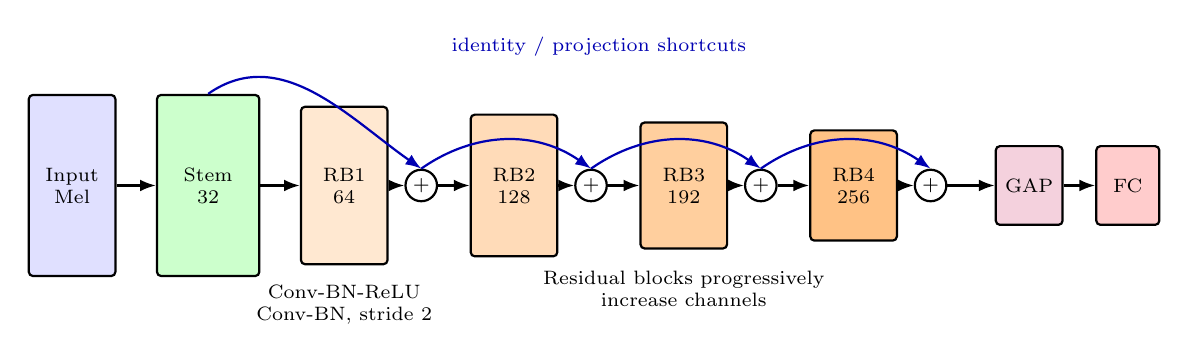
\begin{tikzpicture}[
  node distance=6mm and 5mm,
  every node/.style={font=\scriptsize},
  stage/.style={draw=black, rounded corners=1.5pt, thick, minimum width=11mm, minimum height=20mm, align=center, fill=orange!20},
  stem/.style={draw=black, rounded corners=1.5pt, thick, minimum width=13mm, minimum height=23mm, align=center, fill=green!20},
  io/.style={draw=black, rounded corners=1.5pt, thick, minimum width=11mm, minimum height=23mm, align=center, fill=blue!12},
  head/.style={draw=black, rounded corners=1.5pt, thick, minimum width=8mm, minimum height=10mm, align=center, fill=purple!18},
  plus/.style={circle, draw=black, thick, inner sep=1pt, minimum size=4mm, fill=white},
  arr/.style={-{Latex[length=2mm]}, thick},
  skip/.style={-{Latex[length=2mm]}, thick, blue!70!black}
]
\node[io] (in) {Input\\Mel};
\node[stem, right=of in] (stem) {Stem\\32};

\node[stage, right=of stem, fill=orange!18] (rb1) {RB1\\64};
\node[plus, right=2mm of rb1] (p1) {$+$};
\node[stage, right=4mm of p1, fill=orange!28, minimum height=18mm] (rb2) {RB2\\128};
\node[plus, right=2mm of rb2] (p2) {$+$};
\node[stage, right=4mm of p2, fill=orange!38, minimum height=16mm] (rb3) {RB3\\192};
\node[plus, right=2mm of rb3] (p3) {$+$};
\node[stage, right=4mm of p3, fill=orange!48, minimum height=14mm] (rb4) {RB4\\256};
\node[plus, right=2mm of rb4] (p4) {$+$};

\node[head, right=6mm of p4] (gap) {GAP};
\node[head, right=4mm of gap, fill=red!20] (fc) {FC};

\draw[arr] (in) -- (stem);
\draw[arr] (stem) -- (rb1);
\draw[arr] (rb1) -- (p1);
\draw[arr] (p1) -- (rb2);
\draw[arr] (rb2) -- (p2);
\draw[arr] (p2) -- (rb3);
\draw[arr] (rb3) -- (p3);
\draw[arr] (p3) -- (rb4);
\draw[arr] (rb4) -- (p4);
\draw[arr] (p4) -- (gap);
\draw[arr] (gap) -- (fc);

\draw[skip] (stem.north) to[out=35,in=145] (p1.north);
\draw[skip] (p1.north) to[out=35,in=145] (p2.north);
\draw[skip] (p2.north) to[out=35,in=145] (p3.north);
\draw[skip] (p3.north) to[out=35,in=145] (p4.north);
\node[skip, draw=none] at ($(rb2.north)!0.5!(rb3.north)+(0,9mm)$) {identity / projection shortcuts};

\node[align=center] at ($(rb1.south)+(0,-5mm)$) {Conv-BN-ReLU\\Conv-BN, stride 2};
\node[align=center] at ($(rb3.south)+(0,-5mm)$) {Residual blocks progressively\\increase channels};
\end{tikzpicture}
\caption{Residual CNN architecture (\texttt{residual\_cnn}) with skip connections in each residual block.}
\label{fig:arch-residual}
\end{figure}

\subsection{Optimization and Training}
Training uses AdamW for optimization with 35 epochs and batch size 64. To address imbalance, we enable both a balanced sampler and focal loss, following the intuition that hard or minority examples should receive more learning emphasis. Early stopping is driven by validation Macro-F1, and posthoc calibration and tuning are enabled to improve score reliability.

This recipe explicitly balances convergence speed and generalization. The optimizer and weight decay values are held constant across variants to control confounding factors, while augmentation is switched in targeted runs to test robustness gains. By keeping these controls explicit, downstream conclusions about architecture choice are stronger and easier to defend.

\subsection{Serving/Consumption}
For model consumption, we provide a lightweight batch inference artifact. The script \texttt{predict\_genre.py} loads a trained checkpoint and outputs top-K genre probabilities in JSON format. The inference utility now supports architecture-aware checkpoint loading, which allows a single script to consume both residual and standard CNN checkpoints without manual model edits. This reduces operational friction when comparing candidate models or rolling back to a prior version.

\subsection{End-to-End Pipeline Diagram}
\begin{figure}[H]
\centering
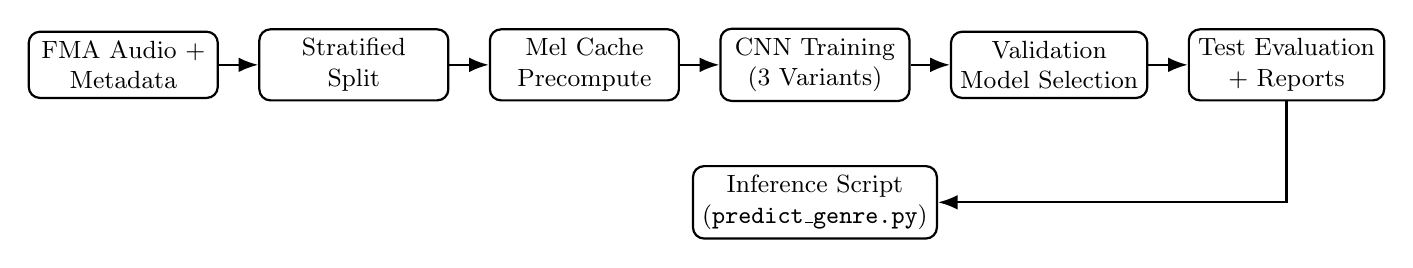
\begin{tikzpicture}[
  node distance=8mm and 5mm,
  every node/.style={font=\small},
  block/.style={rectangle, rounded corners, draw=black, thick, align=center, minimum height=8mm, minimum width=24mm},
  arrow/.style={-{Latex[length=2.5mm]}, thick}
]
\node[block] (data) {FMA Audio +\\Metadata};
\node[block, right=of data] (split) {Stratified\\Split};
\node[block, right=of split] (cache) {Mel Cache\\Precompute};
\node[block, right=of cache] (train) {CNN Training\\(3 Variants)};
\node[block, right=of train] (val) {Validation\\Model Selection};
\node[block, right=of val] (test) {Test Evaluation\\+ Reports};
\node[block, below=of train] (serve) {Inference Script\\(\texttt{predict\_genre.py})};

\draw[arrow] (data) -- (split);
\draw[arrow] (split) -- (cache);
\draw[arrow] (cache) -- (train);
\draw[arrow] (train) -- (val);
\draw[arrow] (val) -- (test);
\draw[arrow] (test) |- (serve);
\end{tikzpicture}
\caption{End-to-end ML pipeline used in this project.}
\label{fig:pipeline}
\end{figure}

\section{Experiments and Evaluation}
\subsection{Evaluation Metrics}
For this classification problem, we report Accuracy, Macro Precision, Macro Recall, and Macro F1. We prioritize Macro F1 for model selection because it is more sensitive to minority-class behavior under class imbalance. Weighted variants are also retained in run artifacts for diagnostics, but they are not used as the primary decision criterion because they can over-represent high-support classes.

\subsection{Shared Training Protocol}
All three comparison runs use the same split policy, seed, and most optimization settings to make metric differences attributable to architecture and recipe changes rather than data leakage or protocol drift. Table \ref{tab:protocol-summary} summarizes the shared setup and variant-specific changes.

\begin{table}[H]
\centering
\caption{Shared protocol and variant-level differences for CNN comparison runs.}
\label{tab:protocol-summary}
\resizebox{\textwidth}{!}{
\begin{tabular}{lccc}
\toprule
Setting & cnn\_standard\_base\_fullprotocol & cnn\_residual\_fullprotocol & cnn\_standard\_aug\_fullprotocol \\
\midrule
Split strategy / ratios & stratified / 0.8, 0.1, 0.1 & stratified / 0.8, 0.1, 0.1 & stratified / 0.8, 0.1, 0.1 \\
Seed / epochs / batch size & 42 / 35 / 64 & 42 / 35 / 64 & 42 / 35 / 64 \\
Optimizer / LR / weight decay & AdamW / 7e-4 / 1e-4 & AdamW / 7e-4 / 1e-4 & AdamW / 7e-4 / 1e-4 \\
Model architecture & standard\_cnn & residual\_cnn & standard\_cnn \\
Augmentation & disabled & enabled & enabled \\
Balanced sampler + focal loss & enabled & enabled & enabled \\
Posthoc tuning objective & f1\_macro & f1\_macro & f1\_macro \\
\bottomrule
\end{tabular}
}
\end{table}

\subsection{Model Comparison (Main Results)}
\begin{table}[H]
\centering
\caption{CNN comparison under a shared full protocol.}
\label{tab:model-comparison}
\resizebox{\textwidth}{!}{
\begin{tabular}{lcccccc}
\toprule
Model & Val Acc & Val F1$_{macro}$ & Test Acc & Test Prec$_{macro}$ & Test Rec$_{macro}$ & Test F1$_{macro}$ \\
\midrule
cnn\_standard\_base\_fullprotocol & 0.5385 & 0.3624 & 0.5352 & 0.4003 & 0.4180 & 0.3536 \\
cnn\_residual\_fullprotocol & \textbf{0.6698} & \textbf{0.5733} & \textbf{0.6780} & \textbf{0.6135} & \textbf{0.5974} & \textbf{0.5909} \\
cnn\_standard\_aug\_fullprotocol & 0.5610 & 0.4141 & 0.5511 & 0.4046 & 0.4771 & 0.4009 \\
\bottomrule
\end{tabular}
}
\end{table}

\subsection{Key Diagnostic Figures}
The report includes three core visual diagnostics. First, the per-epoch metric curves show training dynamics and whether improvements are stable over time. Second, the model-level metric comparison chart summarizes the final test performance differences across the three CNN variants. Third, the normalized confusion matrix shows which classes are most frequently confused on the test split.

Together, these figures provide complementary evidence: curves establish optimization behavior, aggregate bars establish headline ranking, and confusion patterns establish class-level risk. This prevents over-reliance on a single scalar metric and improves the quality of model-selection decisions.

\begin{figure}[H]
\centering
\includegraphics[width=0.98\textwidth]{../outputs/cnn_variant_res_fullprotocol/metric_curves.png}
\caption{Training and validation metric curves for \texttt{cnn\_residual\_fullprotocol}.}
\label{fig:metric-curves}
\end{figure}

\begin{figure}[H]
\centering
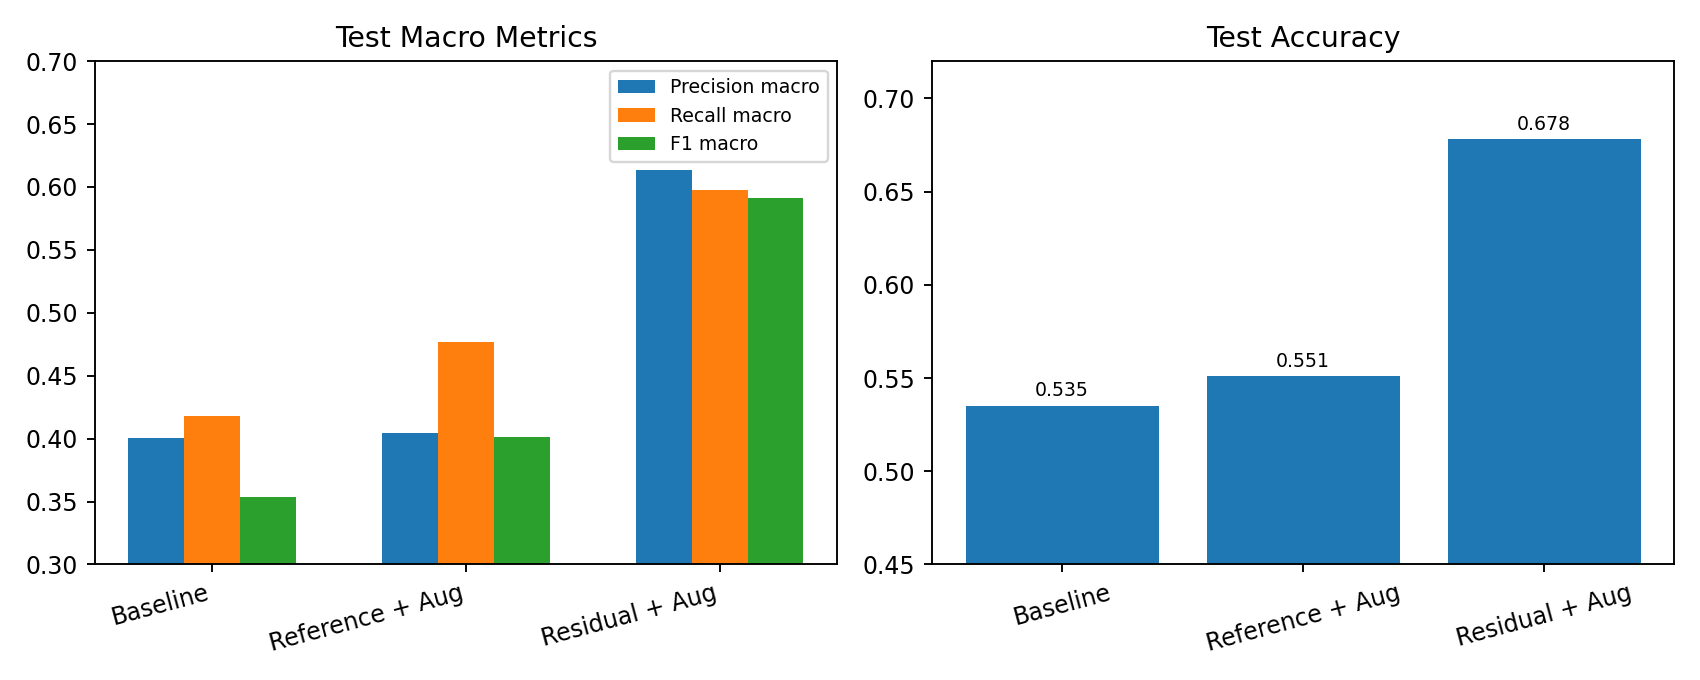
\includegraphics[width=0.94\textwidth]{model_comparison_metrics.png}
\caption{Test-set metric comparison across CNN variants (Accuracy, Precision$_{macro}$, Recall$_{macro}$, F1$_{macro}$).}
\label{fig:f1-pr}
\end{figure}

\begin{figure}[H]
\centering
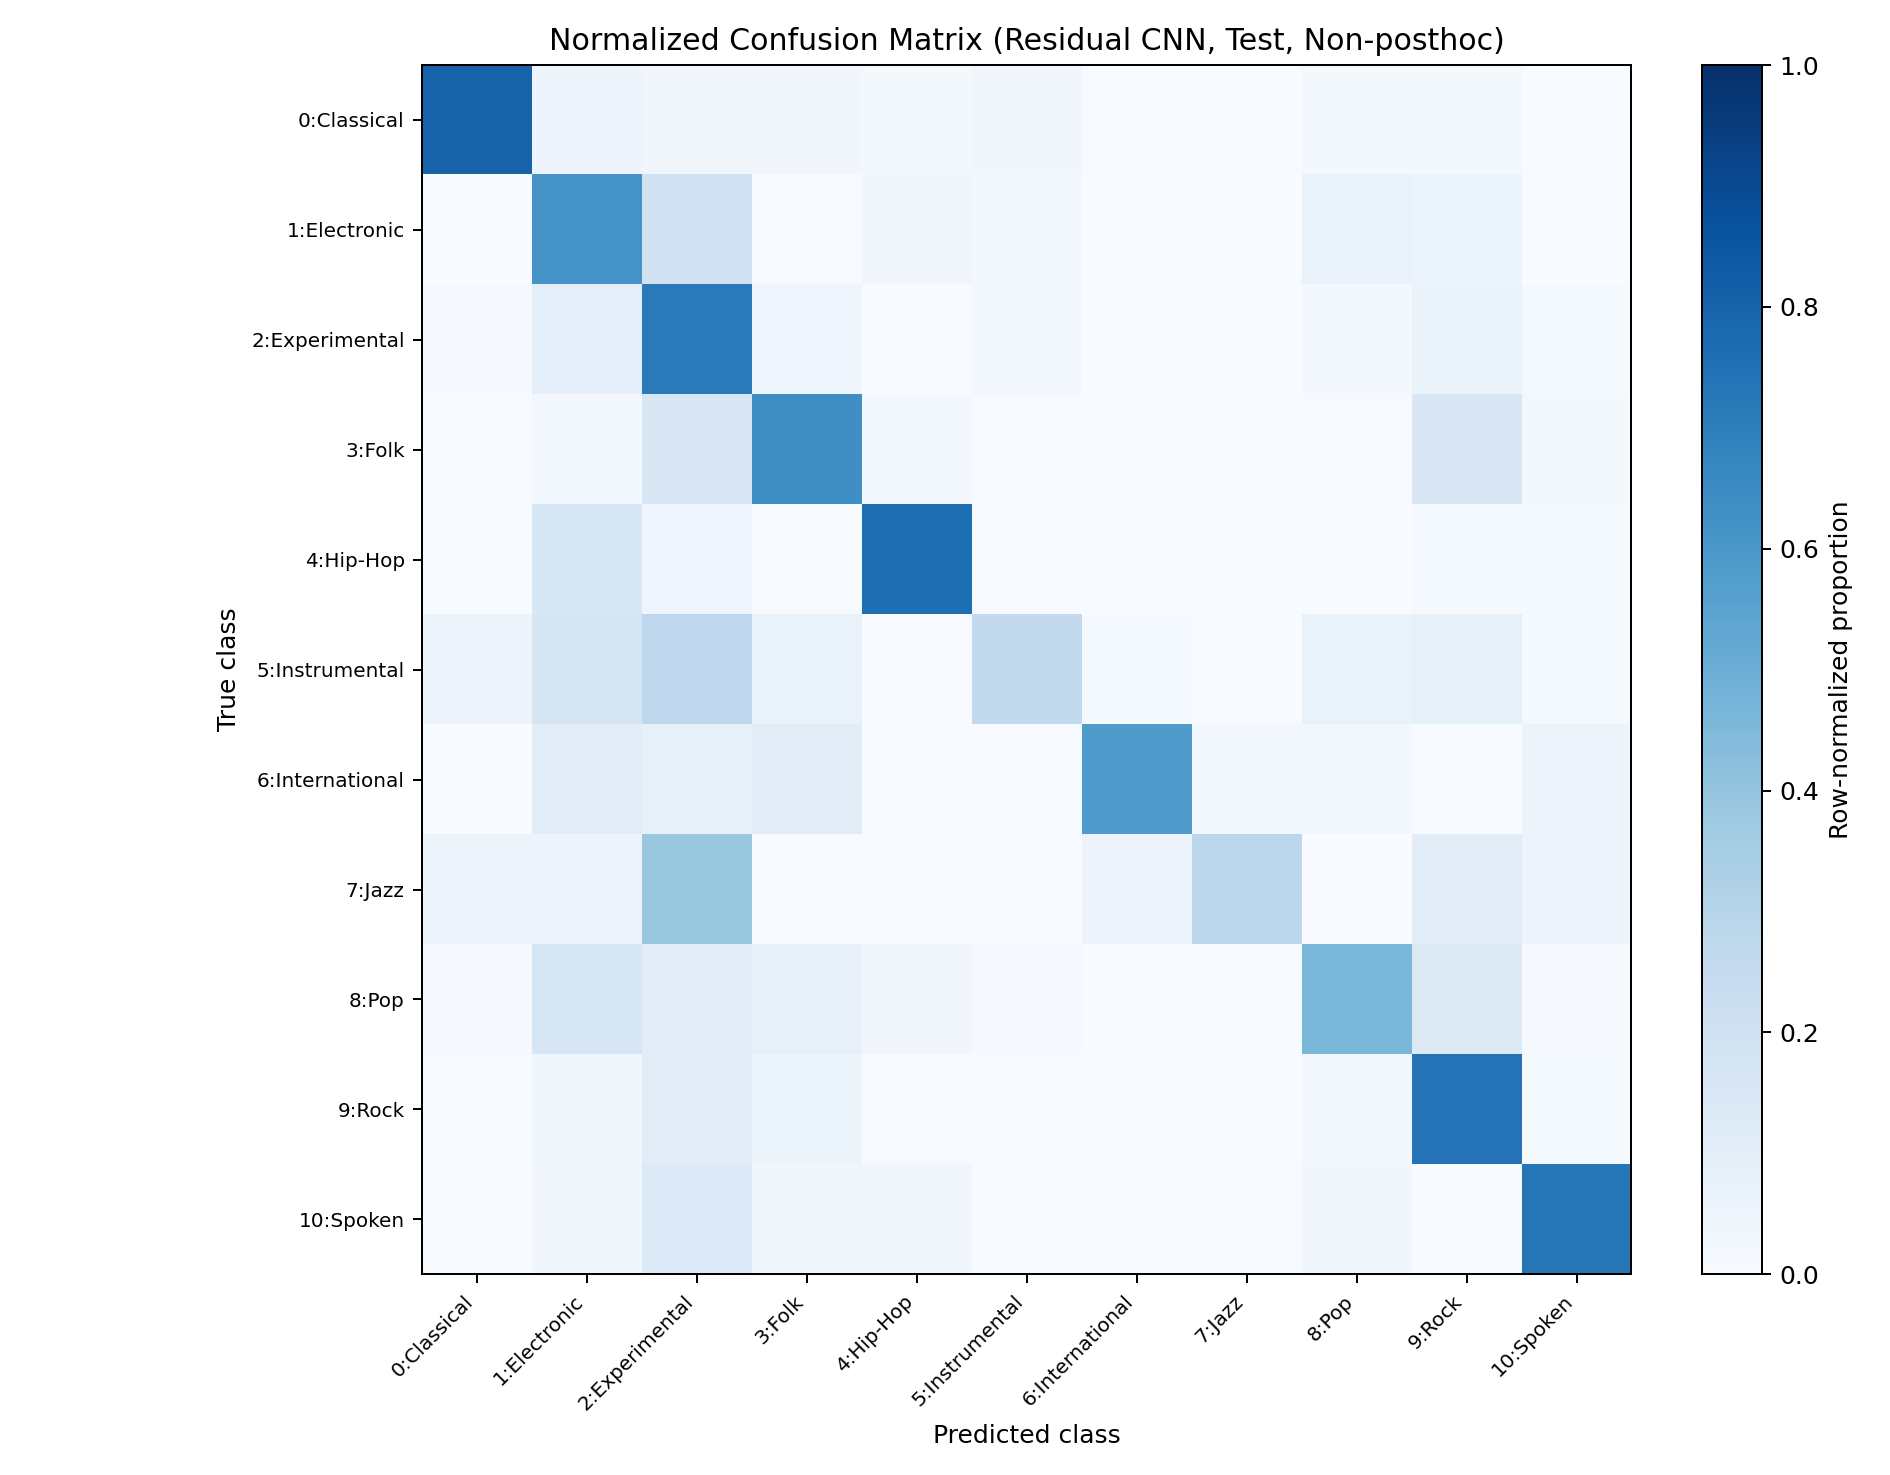
\includegraphics[width=0.84\textwidth]{confusion_matrix_res_fullprotocol.png}
\caption{Row-normalized non-posthoc test confusion matrix for \texttt{cnn\_residual\_fullprotocol}, aligned with the main results table.}
\label{fig:confusion}
\end{figure}

\subsection{Class Index Legend for Confusion Matrix}
For interpretability, the class indices used in Figure \ref{fig:confusion} are mapped as follows: 0 = Classical, 1 = Electronic, 2 = Experimental, 3 = Folk, 4 = Hip-Hop, 5 = Instrumental, 6 = International, 7 = Jazz, 8 = Pop, 9 = Rock, and 10 = Spoken. We include this mapping directly in the report to keep matrix interpretation self-contained and reduce ambiguity during review.

\subsection{Baseline and Hyperparameter Comparison}
The baseline model (\texttt{cnn\_standard\_base\_fullprotocol}) uses the standard CNN with reduced regularization/augmentation and is consistently outperformed by the residual variant. This demonstrates the value of both architecture and training strategy choices. Hyperparameter differences were kept minimal to isolate architecture/training recipe effects under the same data protocol.

The comparison between \texttt{cnn\_standard\_aug\_fullprotocol} and \texttt{cnn\_standard\_base\_fullprotocol} indicates that recipe improvements alone can improve outcomes, but not enough to match the residual architecture. This supports selecting \texttt{residual\_cnn} as the primary model family for future tuning.

\subsection{Bias and Failure Audit}
We observed uneven performance across classes, with better metrics on high-support genres and weaker performance on low-support or semantically overlapping genres. This is expected under class imbalance and noisy boundaries. The normalized confusion matrix in Figure \ref{fig:confusion} highlights repeated error patterns and supports class-level failure analysis.

From a risk perspective, these patterns imply that deployment quality should be monitored at the class level rather than only with global accuracy. In particular, semantically adjacent genres should be tracked for confusion-rate drift, and alert thresholds should be tuned to prioritize user-visible degradation.

\section{Discussion of Results}
The residual CNN variant is the most robust model by both validation and test Macro-F1. The standard CNN can reach moderate performance but is less stable, especially without augmentation. Posthoc tuning slightly improves all models, with the residual variant remaining best. The gap between Macro-F1 and weighted metrics confirms that minority genres remain more challenging than majority classes.

A key practical observation is that the best-performing run is not only better at a single endpoint metric, but also more consistent across diagnostic views. This consistency is important for production adoption because it reduces the chance that gains are due to chance split behavior or transient optimization effects.

\section{Recommendations}
We recommend using \texttt{cnn\_residual\_fullprotocol} as the final selected model because it provides the strongest and most consistent Macro-F1 across validation and test sets. Multi-crop evaluation should remain in offline validation and test-time reporting because it reduces variance from single-crop predictions. The class-imbalance controls should be retained, specifically the balanced sampler and focal loss combination, since they support minority-class performance. After deployment, class-level drift and quality should be monitored continuously to detect degradation early.

Operationally, we recommend a staged rollout with shadow evaluation before full traffic exposure. During rollout, monitor both confidence calibration and per-class confusion profiles. If drift is detected, trigger a retraining cycle using the same reproducible protocol so that new and old models remain directly comparable.

\section{Limitations and Future Work}
Current performance is constrained by dataset label noise and genre overlap, which limit the achievable upper bound for single-label classification. Minority classes remain harder because support is uneven across genres, and audio corruption in source files adds additional preprocessing noise. 

Future work should evaluate stronger audio encoders under a controlled compute budget to improve representation quality, including transfer-learning setups with pretrained audio backbones \cite{hershey2017cnn}. We also plan to introduce calibrated confidence thresholds for abstention so that low-confidence predictions can be flagged for review. Data-centric improvements, including targeted cleaning, class-aware augmentation, and rebalancing strategies, are likely to produce additional gains.

Another priority is richer labeling objectives. Because many tracks may plausibly span multiple stylistic categories, a future multilabel formulation may better match semantic reality than strict single-label prediction. This would require revised evaluation and business acceptance criteria, but may reduce confusion among related genres.

\section{References}
\begin{thebibliography}{9}
\bibitem{defferrard2017fma}
Micha\"el Defferrard, Kirell Benzi, Pierre Vandergheynst, and Xavier Bresson.
\newblock FMA: A Dataset for Music Analysis.
\newblock In \textit{18th International Society for Music Information Retrieval Conference (ISMIR)}, 2017.

\bibitem{he2016resnet}
Kaiming He, Xiangyu Zhang, Shaoqing Ren, and Jian Sun.
\newblock Deep Residual Learning for Image Recognition.
\newblock In \textit{Proceedings of the IEEE Conference on Computer Vision and Pattern Recognition (CVPR)}, 2016.

\bibitem{choi2017transfer}
Keunwoo Choi, George Fazekas, Mark Sandler, and Kyunghyun Cho.
\newblock Transfer Learning for Music Classification and Regression Tasks.
\newblock In \textit{18th International Society for Music Information Retrieval Conference (ISMIR)}, 2017.

\bibitem{hershey2017cnn}
Shawn Hershey et al.
\newblock CNN Architectures for Large-Scale Audio Classification.
\newblock In \textit{IEEE International Conference on Acoustics, Speech and Signal Processing (ICASSP)}, 2017.
\end{thebibliography}

\section{Reproducibility Appendix}
\subsection{Environment}
\begin{verbatim}
python3 -m venv .venv
source .venv/bin/activate
pip install -r requirements.txt
\end{verbatim}

\subsection{Run Commands}
\textbf{CNN model comparison (full protocol):}
\begin{verbatim}
PATH="$(pwd)/.venv/bin:$PATH" bash scripts/run_cnn_comparison.sh
\end{verbatim}

\textbf{Single-file inference demo:}
\begin{verbatim}
python predict_genre.py fma_large/002/002003.mp3 \
  --checkpoint outputs/cnn_residual_fullprotocol/best_model.pt --top-k 5
\end{verbatim}

\subsection{Figure/Table Reproduction Map}
\begin{longtable}{>{\raggedright\arraybackslash}p{0.30\textwidth} >{\raggedright\arraybackslash}p{0.65\textwidth}}
\toprule
Artifact in report & Reproduction source \\
\midrule
Pipeline diagram (Fig. \ref{fig:pipeline}) & Embedded TikZ in this \texttt{.tex} file \\
Model comparison table (Table \ref{tab:model-comparison}) & \texttt{outputs/*\_fullprotocol/summary.json} \\
Training curves (optional figure) & \texttt{outputs/<run>/metric\_curves.png} generated by training script \\
Model-level metric comparison figure & \texttt{docs/model\_comparison\_metrics.png} generated from full-protocol \texttt{summary.json} files \\
Confusion matrix analysis & \texttt{outputs/<run>/test\_confusion\_matrix.npy} \\
\bottomrule
\end{longtable}

\subsection{Deployment Monitoring Requirements}
If this model is deployed as a service, monitoring should include latency at P50, P95, and P99; throughput measured in requests per second; data drift across duration, sample-rate, and loudness distributions; and prediction drift tracked through per-class output distributions over time.

\subsection{Team Contributions}
\begin{table}[H]
\centering
\caption{Team contribution summary (fill before submission).}
\begin{tabular}{lll}
\toprule
Member & Responsibility & Deliverables \\
\midrule
Ang Kar Kin & Data + preprocessing & split policy, cache precompute, quality checks \\
Nicolas Lasch & Modeling + experiments & architecture variants, tuning, evaluation \\
Nisal Jinadasa & Reporting + deployment demo & report, presentation, inference artifact \\
\bottomrule
\end{tabular}
\end{table}

\subsection{Submission Checklist Pointers}
Before final upload, confirm that the report PDF is present in the repository, code and notebooks are documented, dataset and large weights are provided via external link if needed, and reproducibility commands have been validated end-to-end.

\end{document}
